\FloatBarrier
\subsubsection{Main control and alignment strategies}\label{sec:control}
%\emph{Author(s):  C.\ Graef, M.\ Mantovani, S.\ Hild \\}
%\begin{itemize}
%\item{Maybe refer to aLIGO locking scheme T070247-01}
%\item{filter cavity locking scheme, with link to Sec.~\ref{sec:filtercavities}}
%\item{\dots}
%\end{itemize}

%\subsubsection{Fundamentals of length sensing and control}\label{sec:fundamentals_of_lsc}
As a matter of fact, in interferometric GW detectors---the highly complex optical instruments they have grown---it is a crucial requirement 
for the multitude of their degrees-of-freedom (DOF) that they are held tightly at predefined operating points, for instance to allow for full internal power build 
up or to enable active null operation. 
For keeping the mirrors at their operating positions, electronic feedback control has proven as an essential tool, 
making a deterministic and reliable operation 
of a GW detector possible.

\etbox{h}{hbox:sensing_and_control}{Interferometric sensing and control for ET}
{
The configurations of the ET main interferometers, featuring a dual-recycled Michelson interferometer
with Fabry-Perot cavities in the arms, has been chosen to be similar to 
Advanced LIGO and Advanced Virgo.  In addition the reflectivities and the resulting cavity finesse for 
the arm cavities and the recycling cavities will be within a factor of two of what is planned for the second 
generation interferometers. These choices have been made  consciously  in order to be able to transfer
as much as possible the interferometric sensing and control concepts developed and implemented in second generation Gravitational wave detectors
to ET. 
}

The task of controlling an interferometer can further be sub-divided in the control of longitudinal DOF and alignment control.
In the following we will first focus on aspects of controlling the longitudinal degrees of freedom  (i.e.\ only variations along the axis of the optical mode in the interferometer
will be considered) and in the later part discuss alignment control.%will be treated in Section~\ref{sec:asc}.
\FloatBarrier
\paragraph{Fundamentals of length sensing and control}%\label{sec:fundamentals_of_lsc}

A successful length sensing and control system for ET has to satisfy three basic requirements: First, starting from a random 
initial state it must bring the instrument to a predefined operating point (``lock acquisition''). Second, it must prevent disturbances of any
kind from causing deviations of the instrument from its operating point by an amount larger than specified. Finally, it must provide a low-noise electronic signal which contains the GW signal.
In this discussion we will focus on the first two aspects, while the GW readout has already been discussed in section~\ref{sec:detection}.

A crucial element of a succesful longitudinal control scheme is the extraction of a complete set of signals which reflect 
the dynamical state of the longitudinal degrees-of-freedom and which, in particular, are 
a measure for the deviation of each of the interferometric degrees-of-freedom from its desired operating point.
Generally, this is achieved by employing variants of the fundamental Pound-Drever-Hall technique \cite{DHKHF83}.
The Pound-Drever-Hall scheme builds on imprinting radio-frequency (RF) phase modulation sidebands on the carrier beam prior to its injection into
the optical cavity to be controlled. Cavity length fluctuations are efficiently converted to carrier phase shifts, which occurs near resonance as a linear
effect. The RF sidebands in contrast do not experience a phase shift, as their frequencies are generally chosen off-resonant in the cavity. Pure phase 
modulation is thus partially converted to amplitude modulation. Heterodyne readout of the reflected beam provides a signal which is a direct 
measure for the cavity's deviation from resonance and which can further serve as an error signal for electronic feedback controls.

Ideally, a sensing system would provide a number of independent outputs, one for each DOF in the detector. However, in practice error signals
obtained from an interferometer by means of heterodyne detection show more or less strong coupling. 
This is acceptable as long as these signals are at least linearly independent, due to the fact that this class of signals can be electronically post-processed,
i.e.\ linearly transformed, resulting in separated signals. The underlying transforms can easily be implemented in the form of matrices in digital data processing systems. 
However, care must be taken to provide rubustness of the transformations under parameter changes of the optical plant and the sensing electronics. This is why in practice optically
separated signals are usually preferred over signals obtained via electronic separation. 
Further potential disadvantages of electronically separated signals are a reduced signal-to-noise ratio and more complex dynamics during lock acquisition~\cite{SKKKS07}.
Generally, providing too few modulation frequencies or extraction ports complicates the task of finding a set of independent length signals and, in the worst case,
leaves the optical system underconstrained due to a lack of information about its internal state.

A valuable form of description for the design of a sensing scheme is the \emph{sensing matrix}.
The sensing matrix describes the relation between the interferometer's degrees-of-freedom and the signal extraction ports. In the ideal case
this matrix would be diagonal which would read as all sensing signals being fully decoupled. Likewise, the control problem would decouple to a single-input single-output
problem for each degree-of-freedom in the interferometer. Contrasting this, the  signal mixing of length error signals one encounters in practice would yield non-vanishing off-diagonal elements in the sensing matrix.
This is tolerable, as long as the off-diagonal elements are smaller in magnitude than the diagonal ones as in this case a technique referred to as \emph{gain hierarchy}
can be applied to solve the control problem. This technique is based on suppressing a large signal that appears in more than one port by closing a control loop around the DOF that causes it. 
A small signal, previously covered by the large one, can in this way be dissected from the signal mixture and serve as an error signal for another, by then uncontrolled, degree-of-freedom. 

The classical approach of implementing servo controllors by means of analog electronics is driven from predominance more and more by digital control systems. At the expense of their higher cost and obvious bandwidth limitation,
digital systems provide a high precision and low noise environment allowing for rapid design and easy duplication of solutions. Massively multiple-input multiple-output systems become feasible and
instrument automation can be easily implemented. Unlike analog electronics digital servo systems exhibit a high immunity to environmental parameter changes which makes them predestinated for applications
which require long-term stable operation. Despite all these obvious advantages, it is fair to say that digital system complexity, in practice, rivals analog controls. 
\FloatBarrier
\paragraph{Longitudinal sensing and control in Advanced generation detectors}%\label{sec:review_adv_generation_lsc}
With increasing complexity and a growing number of degrees-of-freedom in the instruments comes the need for highly sophisticated length sensing and control schemes, which  
are substantial to setting the detector into operation.
The interferometric topology that will be adopted by the Einstein Telescope is the cavity-enhanced dual recycling Michelson interferometer, 
which is also the underlying topology of the Advanced GW observatories currently under construction.
In this section a review of central aspects of the sensing and control concepts of a typical Advanced generation GW observatory is given, focussing on Advanced LIGO~\cite{AdvancedLIGO} as an example. 
The optical setup is schematically depicted in Fig.~\ref{Fig:Sec_Optics_AdvLIGO_IFO_Schematic}.

\begin{figure}[th]
\centering
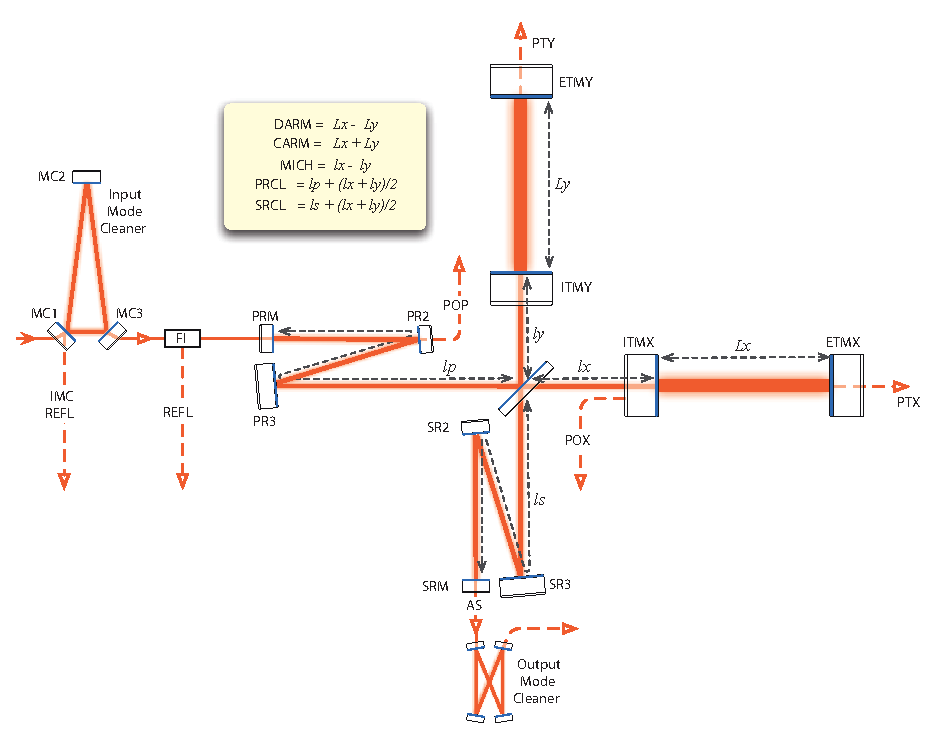
\includegraphics[width=0.8\textwidth]{Sec_Optics/aLIGO_IFO_Schematic}
\caption[Schematic optical layout of Advanced LIGO]
{Schematic drawing of the Advanced LIGO optical layout, degrees-of-freedom and sensing ports \cite{aLIGO_lscfdd}. 
Error signals for the control of the five longitudinal degrees-of-freedom are extracted from the four ports REFL, AS, POP and POX.}
\label{Fig:Sec_Optics_AdvLIGO_IFO_Schematic}   
\end{figure}

For Advanced LIGO different modes of operation are foreseen, each of them involving e.g.\ different input laser power levels, signal
recycling tunings, homodyne detection phases, etc., to yield optimum signal-to-noise ratio, depending on the astrophysical source under investigation~\cite{aLIGO_lscfdd}. 
The main differential control requirement for Advanced LIGO is $10^{-15}$\,m rms, yielding a shot noise limited sensitivity of $4 \times 10^{-21}$\,m/$\sqrt{\textnormal{Hz}}$.

At the detector's operating point the carrier laser light is resonant in the power recycling cavity (PRC) and in the arm cavities. The signal recycling cavity (SRC)
is tuned to carrier resonance only if the detector is operated in tuned mode. 
Two pairs of phase modulation sidebands, locked by a PLL, are imprinted on the input laser, forming the basis of the sensing scheme. 
The frequencies were chosen to be $f_1=9$\,MHz and $f_2=45$\,MHz, both nearly anti-resonating in the arms to reduce arm-cavity induced phase shifts.%\footnote{This turns out
%to have a positive effect on the shot noise sensitivity of the Michelson (MICH) degree-of-freedom.} 
Both pairs of modulation sidebands are resonant in the power recycling cavity. The signal recycling cavity, however, is arranged to be nearly resonant for the $f_2$ sidebands 
while the $f_1$ sidebands do not resonate.

A typical property of the recycling cavities is their potential to cause mixing of modulation sidebands which immediately leads to 
coupled error signals. To prevent this effect from rendering the control scheme more complicated than necessary it is crucial to 
arrange for a configuration that reduces this mixing to the largest possible extent. 

The Schnupp asymmetry---a macroscopic offset in the arm lengths of the central Michelson---is set to 5\,cm to provide nearly critical coupling of the $f_2$ 
sidebands in the dual recycling cavity, with the implication of simultaneous resonance of the power recycling and the signal recycling cavities 
for this sideband frequency. By choosing an appropriate value for the Schnupp asymmetry one can arrange for a large modulation sideband power ratio in the SRC, 
providing improved signal separation. In this case the resulting power ratio is of the order of $10^3$, in favor of the $f_2$ sidebands.

A variety of ports in the interferometer are read out to obtain a complete set of control signals for all longitudinal degrees-of-freedom. 
Besides the asymmetric port (AS), signals are extracted from the symmetric port (REFL) and from pick-off ports from within the power recycling cavity (POP)
and a in reflection of one of the arm cavities (POX). These beams are directed to photodetectors and the resulting signals are in 
turn demodulated at $f_1$, $f_2$, $f_2-f_1$ or $f_1+f_2$, at appropriately set demodulation phases. 
Demodulation at the sum or difference frequency of two modulation sidebands, i.e.\ at their beat frequency, is a key concept in modern interferometric control system design and is 
often referred to as \emph{double demodulation}.

The signal obtained in the symmetric port, after demodulation at the lower sideband frequency $f_1$ is used for common mode arm cavity (CARM) control. 
Consequently, the differential arm cavity mode control signal is obtained in the asymmetric port from the AS DC photodetector. For the DC readout scheme 
of the asymmetric port, which also contains the GW signal, a differential arm length (DARM) offset of the order of $10^{-11}$\,m will be applied, yielding a DC power level in 
the asymmetric port of the order of $0.1$\,W of carrier light.
The intra-cavity POP port yields signals for the PRC and the Michelson degrees-of-freedom, after demodulation at
$f_1$ and $f_2$, respectively. 

For controlling the signal recycling cavity, the optimum signal extraction port as well as the demodulation frequency depends on the mode of operation, i.e.\ the tuning 
of the SR cavity. Whereas for zero detuning an appropriate error signal can be extracted in the symmetric port in reflection of the
interferometer or at the arm cavity pick off port, for detuned operation analyses have shown that double demodulation of the asymmetric port signal
yields better error signals. Thus, if it is desired to continuously tune the SR from tuned mode to a detuned science mode, at a detuning of about
5 deg it is necessary to switch between error signals for the control of the signal recycling cavity.

The underlying sensing matrix shows well-separated error signals for the arm cavities' degrees-of-freedom. The power recycling cavity is sufficiently decoupled from the other degrees-of-freedom
but shows strong coupling to the ports where the Michelson and signal recycling cavity error signals are obtained. The most worrisome degrees-of-fredom are the differential arm length of the central Michelson interferometer (MICH) and the signal recycling
cavity length which exhibit comparably large amount of cross-coupling. However, control of the interferometer can be gained e.g.\ with a gain hierarchical approach in conjuction with the arm length stabilization system (ALS) which
is discussed in Sec.~\ref{sec:detector_lock_acquisition}.

The control signals derived from the error signals are applied to the end mirrors in the case of the DARM degree-of-freedom, to the beamsplitter for differential arm length of the central Michelson feedback  and to the recycling
mirrors for SRC and PRC length stabilization. However, the common mode arm cavity length control loop is the most elaborate one. The CARM error signal is fed back to the main laser via multiply cascaded
frequency loops, providing the final level of frequency correction.
The required unity gain frequencies of the servo controllers are of the order of tens of Hz for PRC, SRC and MICH, hundreds of Hz for 
DARM and tens of kHz for the CARM degree-of-freedom. 

With the exception of the arm cavity common mode controller all servo loops are realized using digital controls.
The more demanding (in terms of bandwidth) CARM servo will be implemented in analog electronics.
The digital feedback loops are implemented in a custom-made real-time control system with typical sampling rates of up to
65536 samples per second at up to 18 bit resolution. Digital control systems have proven to be a powerful solution with high flexibility. 
Complex filter structures, e.g.\ with blending of sensors and signals, can be conveniently realized and changed on-the-fly with little effort.

Similar to the initial LIGO control scheme, correction paths are included in the Advanced LIGO scheme. Correction signals are filtered 
copies of sensing noise limited MICH and SRCL control signals. To cancel the effects of known couplings, correction signals are fed
from SRCL to DARM and from MICH to DARM at a precision of 1\%. An additional correction path will feed signals from PRCL to DARM, at
a lower precision of 10\%.
\FloatBarrier
\paragraph{Detector lock acquisition}\label{sec:detector_lock_acquisition}
Lock acquisition is the process of bringing an interferometer from its uncontrolled, initial state to a controlled state in which the instrument
is fully operable. 
Contrasting the case of a servo loop operating near resonance, where the error signal for an optical cavity shows a linear response to length changes, during lock acquisition one has
to generally deal with highly nonlinear signals. Servo loops are usually optimized for control on resonance, resulting in a poor performance during acquisiton.
The determining quantity in lock acquisition of an optical cavity system are the mirrors' relative velocities. Further, the \emph{threshold velocity} 
is usually referred to as a measure which quantifies the performance of an acquisition scheme. By definition the threshold velocity is the maximal relative velocity of 
two cavity mirrors below which lock acquisition is successful. The threshold velocity strongly depends on the bandwidth of the underlying control loop.
Only if the servo response time is suffiently short to follow the transient error signal it is capable of ``capturing'' an optic.
As the probability for all DOF being simultaneously at their operating points is very small, a sequential approach must be taken, bringing the DOF to the locked state one after another.

The simplistic approach to lock acquisition, e.g.\ practiced in the early detector prototypes, is to wait for the instrument's DOF, driven by random ground motion, to move close to their operating points and then swiftly engage
the control loops. As with this method lock acquisition of an interferometric GW detector would be a pure matter of coincidence more deliberate approaches were strongly desired.
For initial LIGO an acquisition algorithm was developed which is based on a real-time estimate of the time-evolving sensing matrix, derived from measurable signals during lock acquisition \cite{EMFBBGKLSW02}.
With the implementation of this scheme on the LIGO digital control and data system lock of the detector was on average acquired on timescales of $\sim1$\,min. 
The Virgo approach to lock acquisition was to effectively decouple the instrument's DOF which is achieved by a deliberate misalignment of optics. This technique is often referred to as \emph{variable 
finesse locking} \cite{Virgo_VariableFinesse06}. Lock was usually acquired within a few minutes. 

The Advanced LIGO quadruple suspensions provide isolation to the test masses with respect to ground motion at frequencies above 10\,Hz.
Even though the active internal seismic isolation (ISI) platforms provide additional low frequency isolation, low frequency disturbances are
expected to cause significant test mass displacement of the order of $10^{-7}$m/$\sqrt{\textnormal{Hz}}$ at 0.5\,Hz. This is due to the fact that at 
the suspension system's resonance frequency or at lower frequency perturbations are not well attenuated and couple into the test masses' positions as displacement noise.
Besides this, the test masses will have electrostatic actuators instead of coil-magnet actuators which were used in initial LIGO. Electrostatic actuators deliver
lower actuation noise, at the expense of significantly lower actuation force they can exert on the test masses. The Advanced LIGO electostatic actuators are expected to
saturate at forces of $\sim200\,\mu$N \cite{LIGO_T1000294}. This severely complicates the process of lock acquisition.

In order to ease the difficulties of lock acquisition in the Advanced detector generation, auxiliary laser based schemes will be employed to complement the well-established techniques.
This discussion focusses on the Advanced LIGO ALS (arm length stabilization) system \cite{aLIGO_ALS_Design}. For Advanced Virgo it is anticipated to employ a similar scheme. 
Other systems to aid lock acquisition, that were considered for use in Advanced LIGO, such as the suspension point interferometer or digital interferometry are described in \cite{LIGO_T080139}.
The underlying idea of ALS is to provide for more deterministic lock acquisition by locking the arm cavities independently of the remaining degrees-of-freedom.
The ALS system builds on frequency doubled laser beams launched into the arm cavities through the end test masses for pre-stabilization of the interferometer arms,
independent of the science laser circulating in the interferometer. By applying additional coatings on the arm cavity mirrors the properties of the arm cavities, 
as seen from the ALS, can be shaped in accordance to the pre-stabilizations scheme's requirements. The choice of reflectivities for the input mirror and the end mirror 
results in an overcoupled cavity for the auxiliary laser, seen from the end mirror. The Finesse of the arm cavities for the 532\,nm ALS beams is $\sim100$. 
A simplified schematic of the ALS principle setup is depicted in Fig.~\ref{Fig:Sec_Optics_AdvLIGO_ALS_Schematic}.

\begin{figure}[th]
\centering
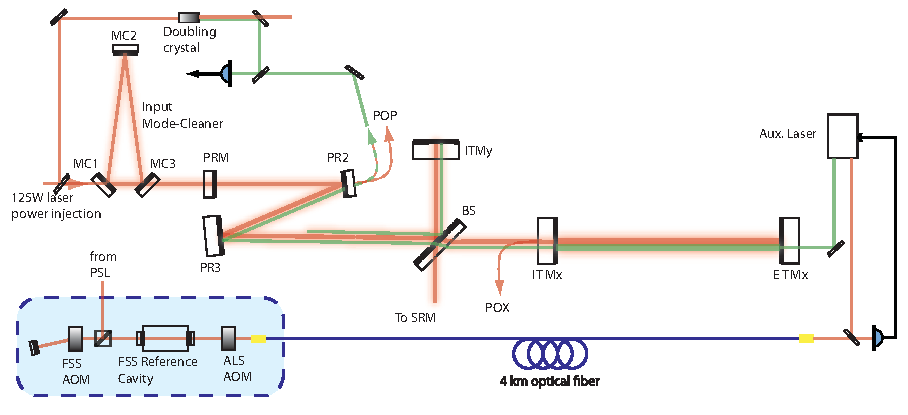
\includegraphics[width=0.8\textwidth]{Sec_Optics/aLIGO_ALS_Schematic}
\caption{Schematic drawing of the Advanced LIGO arm length stabilization (ALS) subsystem \cite{aLIGO_ALS_Design}. The test mass motion is reduced prior to lock acquisition by a combined scheme
of PDH reflection locking of an auxiliary laser to the arm cavities and hetorodyne detection of the transmitted beams. The optical fiber is necessary to provide an optical reference at the end 
stations, to lock the auxiliary lasers' phases to the science laser.}
\label{Fig:Sec_Optics_AdvLIGO_ALS_Schematic}   
\end{figure}

The initial step in the acquisition process is to hold the arm cavities on anti-resonance for the main science laser. In the next step the 
recycling cavities are brought to the locked state, before the ALS brings the arm cavities onto resonance with the main laser and
hands over the control authority to the global interferometer sensing and control scheme. For effectiveness, the ALS must reduce the residual
arm cavity length fluctuations to a displacement of no more than one cavity line width, which is approx. 1.3\,nm in the case of the
Advanced LIGO arm cavities. Estimations have shown that with ALS engaged a level of displacement fluctuations of 0.115\,nm rms can be 
reached. 

Technically, once the arm cavities are locked with the 532\,nm beams, a heterodyne measurement is performed on the ALS beam transmitted by 
the x-arm cavity and a frequency doubled sample of the main laser beam. A second one is performed between the x-arm and the y-arm transmitted beams. These measurements 
yield common and differential mode error signals which are in turn fed back to the corresponding actuators. By introducing a tunable offset
into the heterodyne locking loop, the arm cavities can thus be adjusted to arbitrary tunings.

For a smooth transition from ALS arm cavity control to global control a robust phase-locked loop (PLL) is crucial, to provide a well-defined phase relationship
between auxiliary lasers and the main science laser. Once the PLL is closed, the auxiliary lasers are locked to the arm cavities using PDH reflection locking. The resulting control signal
acts on a voltage-controlled oscillator (VCO) which supplies the electronic local oscillator for the PLL. In this way the offset frequency of the auxiliary laser with
respect to the reference is tuned. An analog servo is foreseen for this loop and is expected to have a bandwidth of a few kHz.

To provide a stable frequency standard for the auxiliary laser PLL, a technique based on the LISA (Laser Interferometer Space Antenna) back-link measurement is employed. Mullavey et al. \cite{MSSM10}
have experimentally demonstrated a scheme based on counter propagating two laser beams through an optical fiber and subsequent measurements of each of the 
outputs with LISA-style phasemeters. By subsequent combination of the output signals an error signal can be obtained which can be utilized to eliminate fiber induced phase noise. Their setup 
consisted of 4.6\,km single mode optical fiber and two Nd:YAG lasers---operated in a master-slave configuration. To circumvent
nonlinear forms of noise such as stimulated Brillouin scattering, the transmitted laser power was reduced to $\sim50\,\mu$W.
In the underlying bench top experiment a relative frequency noise of 0.5\,mHz/$\sqrt{\textnormal{Hz}}$ was reached for Fourier frequencies between 5\,Hz and 20\,Hz which is
well below the Advanced LIGO requirements, with a margin of more than an order of magnitude.


%\section{Introduction}

%The detection principle of a large scale gravitational wave interferometer is to sense the passage of a gravitational wave as a light intensity change at the asymmetric interference port  due to the phase shift in the long arms. 
%This is possible only if the test masses are suspended well enough to be considered as \emph{free-falling test masses}.\\
% Such instruments provide  useful signal only when the optical components are positioned precisely at  pre-defined locations relative to each other (to have the long cavities resonating and a destructive interference at the beam splitter).
% This set of positions is called the \textit{operating point}.\\
% Sophisticated electro-optical feed-back control systems are required to continuously measure and restore the
% mirror positions. Two separate systems to control the mirror position are used: one for the
% longitudinal position along the optical axis, and the other for the angular positions 
% of the mirrors.
\FloatBarrier
\paragraph{Angular control - Automatic Alignment control system}%\label{sec:asc}

The angular control system has to be implemented in order to reduce the mirror misalignments 
in the frequency region in which the seismic attenuation system does not fulfill the alignment
requirements, i.e.\ below the mechanical resonances, to reduce  the fluctuations of the mirror 
angular positions with respect to the beam,  to maintain the overall alignment of the optical elements, 
ensuring long data taking periods, and to reduce the noise at the output
port.
The mirror angular positions in data taking mode can not be locally controlled because the long term 
drifts of the local references spoil the overall alignment.  
After the lock has been acquired the angular control has to be switched to a global control system, the
 \textit{Automatic Alignment},  which uses error signals derived from the interferometer itself with a
 modulation-demodulation technique based on differential wave front sensing.
The control scheme chosen for the second and third generation of gravitational wave interferometer
 is a Ward-like scheme where the RF modulation frequencies are chosen to do not have any 
  higher order modes resonating in the cavities~\cite{ward}.

The main differences between the third generation and the first generation of gravitational wave
 detectors,  relevant for alignment control are: 
 \begin{itemize}
 \item presence stable recycling cavities
 \item higher circulating power
 \item presence of  signal recycling
 \end{itemize}
These modifications will provide an improvement of the overall interferometer stability and sensitivity but also 
increase of complexity for the  Automatic Alignment control system.

\textbf{Stable Recycling cavities issue}

The stable recycling cavities aim to make the potential higher order modes content to be less affected by 
 thermal effects in the mirrors. This behaviour influences the Automatic Alignment control system since the amplitude of 
the alignment error signals is proportional to the amount of the TEM$_{01/10}$ modes. 
For example in the case the recycling cavity with a Gouy phase of 15~deg the TEM$_{01}$ mode is attenuated
 by a factor of about 6 while for 25~deg the attenuation factor is about 9.
For this reason the choice of the recycling cavity Gouy phases has to be done taking into account both the 
stability requirements and the amount of first order higher order modes to ensure the angular controllability of the system. 
 
 
\textbf{High circulating power issue} 

In an high power interferometer \textit{radiation pressure} plays an important role. The light beam acts on the mirror 
such as an optical spring whose strength increases with the power. This effect will be largest in the Fabry-Perot arm cavities,
but the effect has also to be  evaluated for the mirrors of  the central
 interferometer.  

Due to radiation pressure the two cavity mirrors
 become coupled and their angular motion must be described in terms of two linear combinations \cite{sidles-sigg}. 
When the circulating power becomes large enough one of the angular modes can become dynamically unstable. 
As derived in \cite{sidles-sigg}, the interaction of the beam and the mirrors can be written in term of the stiffness matrix:
\begin{equation}
\mathbf{k} = \frac{2PL}{c(1 - g_1 g_2)} \left[ \begin{array}{cc} -g_2 & 1 \\ 1 & -g_1\end{array}\right]
\end{equation}
where $g_i = 1 - L/R_i$ are the G-factors of the two mirrors. The eigenvectors and eigenvalues of the stiffness matrix 
determine the physical angular degrees of freedom and the corresponding stiffness applied to the mechanical system. 

The normal stable situation corresponds to a positive stiffness of the system, given by the contribution of the mechanical 
stiffness of the mirror suspension and the extra-stiffness due to the radiation pressure, which gives a resonance made of
 a pair of complex poles with negative real part and quite large quality factor. The case of negative stiffness instead leads
 to an unstable system described with two real poles, one with positive and one with negative real part, with very close absolute frequency.
The radiation pressure effects have then to be taken into account in the design of the control system.


Moreover the presence of the Signal Recycling mirror increases the number of degrees of freedom to control with respect
 the first generation of gravitational wave interferometers.

The design of the Automatic Alignment control system will be challenging because of the above mentioned issues and of 
the control accuracy and noise requirements to reach the targeted ET sensitivity.
On the other hand all these effects and potential issues will be studied for the commissioning of the second generation 
interferometers, such as Advanced Virgo and Advanced LIGO, and therefore providing plentiful  experience 
how to mitigate these difficulties.

